\documentclass[a4paper]{article}
\usepackage{graphicx} 
\usepackage{hyperref}
\usepackage{booktabs}
\usepackage{listings}
\usepackage{geometry}
\usepackage{booktabs}
\usepackage{multirow}
\usepackage{authblk}

\lstset{
  basicstyle=\ttfamily,
  columns=fullflexible,
  frame=single,
  breaklines=true,
  postbreak=\mbox{{$\hookrightarrow$}\space},
}

\title{Mining experimental data from Materials Science literature with Large Language Models}
\author[1,2]{Luca Foppiano}
\author[1]{Guillaume Lambard}
\author[2]{Toshiyuki Amagasa}
\author[1]{Masashi Ishii}
\affil[1]{Data-driven Materials Research Field, Centre for Basic Research on Materials, NIMS, JP}
\affil[2]{Knowledge and Data Engineering, Centre for Computational Sciences, University of Tsukuba} 

\begin{document}

\maketitle

\begin{abstract}
This work aims to assess the ability of large language models (LLMs) GPT-3.5-Turbo, GPT-4, and GPT-4-Turbo to extract structured information from scientific documents in materials science. 
Addressing the challenge of materials-based information evaluation, we propose a new approach for comparing complex material expressions based on formula normalisation. 
We focus on two key information extraction tasks: named entity recognition (NER) of materials and properties, and relation extraction (RE) between materials and properties. 
We compare the performance of LLMs on these tasks to baseline systems using BERT-based models and rule-based approaches. 
For NER the LLMs fail to outperform the baseline in zero-shot prompting and achieve only marginal gains with few-shot prompting. For RE, GPT-4 and GPT-4 Turbo demonstrate effective reasoning and relation extraction capabilities when given just two examples, outperforming the baseline. 
Overall, the results suggest that while LLMs showcase reasoning abilities in relating concepts, their performance in extracting complex domain entities like materials remains limited compared to small specialised models. 
\end{abstract}

\section{Introduction}

% Why is important?
Mining experimental data from papers has become increasingly popular in materials science due to the vast amount of information available and the need for accelerating materials discovery using data-driven techniques.
A substantial volume of experimental data needs to be gathered, primarily sourced from findings published in scientific articles.
Nonetheless, this data comes in various forms: unstructured textual content and structured tables and graphs, adding complexity to the extraction process. 
As a result, many projects still depend on manual data extraction.
While there are a few extensive structured databases containing accumulated experimental data, they remain limited in number when compared to the numerous projects within the field of materials science research.

% Why is challenging?
In materials science, addressing issues related to data quality and interpretation demands meticulous curation and specialised domain knowledge.
When dealing with scientific texts originating from materials research articles, one must possess a profound comprehension of the laws of physics and the skill to navigate through a maze of jargon, intricate vocabularies, and specialised terminology unique to each sub-domain. 
For instance, in the field of superconductors, experts in the domain categorise materials into classes, which are sometimes defined arbitrarily, blending compound-based classes like \textit{cuprates} and \textit{iron-based} materials with phenomenon-based classes like \textit{fermions}. 
Moreover, there exists substantial confusion due to the frequent overuse of certain terms. For instance, the acronym "TC" is often employed to denote "Temperature Curie," while "Tc" signifies "superconducting critical temperature". 
These sub-domain-specific conventions pose a significant challenge when attempting to create structured datasets that can function effectively across various sub-domains.

% What is the problem we are trying to solve? 
The advent of Large Language Models (LLM) has ushered in a new era of technology with immense potential, ranging from the capacity to link concepts to engaging in conversational reasoning~\cite{zhang2023one,yao2023tree,valmeekam2023planning,sun2023pearl}.
Compared to SLMs, LLMs offer the capability of ingesting more text, working with a context window which is at least 6 to 8 times larger than BERT-base encoders (limited at 512 tokens). 
Furthermore, the interaction with LLMs via prompts changes the construction paradigm which becomes more flexible, and more suitable for human interaction. 
However, the actual capabilities in reasoning, understanding and recognition are still evaluated.

Previous studies in Information Extraction (IE) have shown evidence of LLMs proficiency in general tasks while falling short in areas where specific knowledge is required~\cite{kokon2023chatgpt}. 
In particular, LLMs did not outperform SLMs in most of the discriminative tasks such as named entity recognition (NER), relation extraction (RE) and event detection (ED) in general domains~\cite{ma2023large}, in history~\cite{gonzalez2023yes}, and biology~\cite{moradi2022gpt3}.
Other works testing chemistry capabilities found that GPT-4 understands various aspects of chemistry including chemical compounds~\cite{hatakeyama2023prompt} however, its knowledge is general and lacks methods for learning through retrieving recent literature~\cite{hatakeyama2023using}.

While LLMs present a valuable opportunity to develop more flexible Text and Data Mining (TDM) processes, there is evidence that suggests that in specialised tasks, they are on par with SLMs. 

This study aims to assess LLMs' ability to comprehend, manipulate, and reason with complex information that demands substantial background knowledge as in Materials Science. 

% Goals 
The objectives of this work can be summarised in the following questions: 
\begin{itemize}
    \item \textbf{Q1}: \textit{How effectively can LLMs extract materials science-related information?}
    \item \textbf{Q2}: \textit{To what extent can LLMs engage in reasoning to relate complex concepts?}
    % \item \textit{What volume of information is necessary to use, to bridge the gap between LLMs and specialized SLMs models?}
\end{itemize}

% Method
We observe that the fundamental components of materials science knowledge can be grouped into two main classes: materials and properties expressions. 
Properties (e.g. critical temperature, 4K) are expressed using quantities and measurements: they exhibit a structured format, including modifiers, values, and units, with a wide range of potential values. 
In contrast, materials are conceptually fluid and often depend on the specific domain. They may necessitate a substantial amount of accompanying text for a comprehensive description, which can encompass details like doping ratio, substrate, and other characteristics. 
From a chemical standpoint, materials are defined by their chemical formula. 
However, in practice, scientists frequently employ names such as commercial names, well-known terms, or invented designations to describe samples, all of which serve to streamline information in research papers. Nonetheless, conveying such definitions unambiguously can be challenging.


% NER
To address Q1, we evaluate the LLM's performance on Named Entities Recognition (NER) tasks related to materials and properties extraction.
For each task, we choose a pertinent dataset and analyse the performance of each LLM on that specific dataset.

% The interaction with the LLMs is then performed using three different strategies: zero-shot, few-shot, and fine-tuning (instruct-based generation). 
% For the specific case of few-shot prompting, the way information is provided can be implemented with three strategies: a) provide a definition in the prompt, b) provide examples in the prompt, and, c) provide both. 
% It is crucial to emphasise the significant data requirements for both few-shot and instruct-based generation, for achieving satisfactory results in tasks that involve handling complex vocabulary, particularly in the context of materials science.

% RE
We address Q2 by assessing the capability to establish connections between a predefined set of entities and extract relationships within a given context.  
% The baseline is defined by a rule-based approach we have developed in previous work~\cite{lfoppiano2023automatic}. 
% The interaction with the LLMs is performed only using: zero-shot, few-shot and fine-tuning.  

In both cases, we compare the outcomes against a baseline determined by scores achieved on the same datasets by either a BERT-based encoder or a rule-based algorithm we have developed in previous work.
Our requirement is for the models to be capable of generating output in a valid JSON format as part of our efforts to extract structured databases.
 
% Evaluation matching 
While traditional SMLs classify individual tokens in the input, evaluating their performance against expected datasets involves a straightforward comparison of values. Soft-matching techniques can be employed to overlook minor discrepancies. 
However, with generative models, the output tokens may be structured in ways that significantly differ from the original input sequence. 
In more general scenarios, semantic models that compare the vectorised representations of two sequences can be utilised~\cite{reimers2019sentencebert}. 
Nevertheless, when dealing with concepts like material expressions, a specialised approach is needed. 
As an illustration, the terms "solar cell" and "solar cells" represent identical concepts, yet the materials denoted by "Fe" and "Fn" are entirely distinct, highlighting a difference of just one letter between the two examples.
For this reason, we introduce a novel evaluation method for material names, which involves normalising materials to their chemical formulas before conducting a pairwise comparison of each element. This approach provides a more meaningful and context-aware assessment of the model's performance.

We summarise our contributions as follows: 

\begin{itemize}
    \item We designed and ran a benchmark for LLMs on information extraction, in particular NER of materials and properties. This contribution addresses Q1. 
    \item We evaluated LLMs on RE on entities in the context of materials science. This contribution addresses Q2.
    \item We propose a novel approach for evaluating Information Extraction tasks applied to materials entities which leverage formulas matching via pairwise element comparison.
\end{itemize}


% \section{Related Work}

% Numerous studies have delved into the evaluation of Large Language Models (LLMs) within the scientific domain. However, the rapid advancement in this field poses a significant challenge in synthesising all relevant background studies. Initial assessments of ChatGPT highlighted its proficiency in general tasks, though it fell short in specific areas compared to state-of-the-art (SOTA) models~\cite{kokon2023chatgpt}. In the biomedical domain, the early Curie model struggled to outperform BioBERT in few-shot prompting scenarios~\cite{moradi2022gpt3}.

% A study on correlation and causation detection~\cite{jin2023large} observed that ChatGPT's performance did not surpass that of a random model. Additionally, challenges emerged in named entity recognition and classification (NERC) for historical documents, attributed to potential issues with internet data reliance and inconsistent entity definitions across guidelines~\cite{gonzalez2023yes}.

% In contrast to SLMs like RoBERTa-large, a study~\cite{ma2023large} found that LLMs, including ChatGPT, struggled with tasks such as NER, relation extraction (RE), and event detection (ED) in few-shot prompting scenarios. However, they proposed a hybrid approach, combining both LLMs and SLMs, demonstrating improved performance on tasks requiring specific knowledge or extensive context.

% Another investigation~\cite{tang2023struc} found that GPT3.5-turbo and GPT-4 faced challenges in generating complex output structures like tables, achieving only 3-9\% accuracy on specific formatting constraints. Fine-tuning on a smaller model, significantly improved performance on both seen and unseen structured text generation.
% In materials,~\cite{hatakeyama2023prompt} explored GPT-4’s potential in chemical tasks and other reasoning related to chemical information.

% Notably, the requirement for a valid JSON output, as reported in this study, introduces additional challenges not commonly addressed in related works focused on conversational aspects~\cite{lin2023llmeval, min2023factscore}.


\section{Method}
\label{sec:method}
We chose three OpenAI LLM models: ChatGPT (gpt-3.5-turbo-0611), GPT-4 (gpt-4), and GPT-4-turbo (gpt-4-0611-preview). The consideration of open-source LLMs has been deferred to future work due to their limited capability to generate output in a valid JSON format, necessitating a more in-depth investigation.

Our evaluation is carried out with different strategies: zero-shot learning, few-shot learning and fine-tuning (or instruction-learning).  
Few-shot learning refers to the model's ability to adapt and perform a new task with minimal examples or prompts, while zero-shot learning denotes the model's capability to generalise to tasks it has not been explicitly trained on, emphasising transfer learning within the language domain.
Finally, fine-tuning involves adjusting the parameters of a pre-trained model on a specific task or domain using a smaller, task-specific dataset to enhance its performance for that particular application.

We selected two datasets for evaluation: MeasEval~\cite{harper2021semeval2021}, a SemEval 2021 task of extracting counts, measurements, and related context from scientific documents and SuperMat, an annotated and linked dataset of superconductors research papers~\cite{lfoppiano2021supermat}. 
SuperMat contains both materials and properties and for copyright reasons is not publicly distributed. 
This assures that its annotations had not been seen during the training of any of the LLMs.

Baseline scores were established using a SciBERT-based encoder and RE rule-based algorithm~\cite{lfoppiano2023automatic} for material-related extractions. Grobid-quantities~\cite{foppiano2019quantities} served as the baseline for NER on properties extraction evaluated against MeasEval.

Evaluation scores, encompassing Precision, Recall, and F1-score, were derived from pairwise comparisons between predicted and expected entities. Precision gauges accuracy, recall assesses information capture, and F1-Score harmonises precision and recall.

The presented evaluations condense F1 scores averaged over three extraction runs. Uncertainty is estimated using standard deviation. 
Detailed values are available in the Supplementary Material section.

\subsection{Named Entities Recognition}
\label{sec:ner}
The NER task consists of identifying relevant entities: materials, expressed in a multitude of expressions~\cite{lfoppiano2021supermat}, or properties, expressed as physical quantities and measurements~\cite{foppiano2019quantities}. 

We calculated the evaluation scores using four different matching approaches, although we will present only the most relevant to the task (leaving the complete tables\footnote{The calculation of micro average provides a measure independent of the distribution of the extracted entities over the different documents.} in the supplementary materials section): 
\begin{itemize}
    \item \textbf{strict}: Exact matching
    \item \textbf{soft} Matching using Ratcliff/Obershelp\footnote{\url{https://www.drdobbs.com/database/pattern-matching-the-gestalt-approach/184407970?pgno=5}} with a threshold at 0.9
    \item \textbf{sentence BERT} Comparison using semantic similarity of sequences using Sentence BERT with a cross-encoder~\cite{reimers2019sentencebert}, applying a threshold set at 0.9
    \item \textbf{formula matching} Our novel method compares material expressions via formula normalisation and element-by-element exact matching.
\end{itemize}

Prompts for interacting with LLMs are defined by two components: system and user prompts. 
The system prompt is the initial instruction guiding the model's output generation, defining the task or information sought, while the user prompt is the input from the user, specifying their request and shaping the model's response.

The system prompt remained consistent across all tasks and was specifically crafted to prevent hallucinations and favour standardised negative answers.

\begin{lstlisting}[caption=Generic system prompt common to all requests]
Use the following pieces of context to answer the user's question. 
If you don't know the answer, just say that you don't know, don't try to make up an answer. 
----------------
{text}
\end{lstlisting}


The users' prompts for NER with zero-shot learning were described including the definitions and examples in the SuperMat\footnote{Accessible at \url{https://supermat.readthedocs.io}} and MeasEval\footnote{Accessible at \url{https://github.com/harperco/MeasEval/tree/main/annotationGuidelines\#basic-annotation-set}} annotations guidelines, respectively.  


Following the user prompt templates for both materials and properties extraction: 

\begin{lstlisting}[caption=User prompt designed for extracting materials and properties]
What are the superconductor materials mentioned in the text? 
Only provide the mention of the materials. Avoid repetition. 

The material can be expressed as follows:
- chemical formula with variables not substituted, like La(1-x)Fe(x),
- chemical formula with substitution variables like Zr 5 X 3 (X = Sb, Pb, Sn, Ge, Si and Al)
- with complete or partial abbreviations like (TMTSF) 2 PF 6,
- doping rates are represented as variables (x, y or other letters) appearing in the material names. These values can be used to complement the material variables (e.g. LaFexO1-x).
- doping rates as percentages, like 4% Hdoped sample or 14% Cu doped sample
- material chemical form with no variables e.g. LaFe03NaCl2 where the doping rates are included in the name
- chemical substitution or replacements, like (A is a random variable, can be any symbol): A = Ni, Cu, A = Ni, Ni substituted (which means A = Ni)
- chemical substitution with doping ratio, like (A is a random variable, can be any symbol): A = Ni and x = 0.2

If you don't know the answer, just say you don't know, don't try to make up an answer.

-----

Quantity is either a Count, consisting of a value, or a Measurement, 
consisting of a value and usually a unit. A Quantity can additionally include optional Modifiers like tolerances.
Include relevant text that indicates the application of a modifier, such as "between" "less than" "approximately", 
or symbols such as ">" or "~" if they are contiguous with the span. Ignore them if they are separated by additional text.
 
Example: "The soda can's volume was 355 ml", the quantity is "355 ml".

Extract all the Quantities in the text.
\end{lstlisting}

We implemented the few-shot prompting by reusing the same prompts and injecting a list of suggestions that were extracted from the text using the respective SLM based on the BERT-encoder for materials and properties: grobid-superconductors~\cite{lfoppiano2023automatic}, and grobid-quantities~\cite{foppiano2019quantities}, respectively.
Since the suggestions are provided by another model, they are not correct 100\% of the time, we stressed in the prompt that they are examples or hints, that the LLMs could ignore. 

We applied few-shot learning by incorporating in the prompt templates a set of suggestions derived from the text through the respective SLMs based on materials (grobid-superconductors~\cite{lfoppiano2023automatic}) and properties extraction (grobid-quantities~\cite{foppiano2019quantities}). 
As these suggestions originate from another model, they may not be entirely accurate; hence, we emphasised in the prompts that they serve as examples or hints and can be disregarded: 

\begin{lstlisting}[caption=Few-shot learning modified prompt template.]
[...]
Here are some examples appearing in the text: {hints}
[...]
\end{lstlisting}

For all tasks, we required a valid JSON response. The JSON format was obtained by adding formatting instructions in the prompt based on the expected output data model. 
We used the implementation provided by the LangChain library~\footnote{\url{https://github.com/langchain-ai/langchain}} of which one example is illustrated in the following listing. 

\begin{lstlisting}[caption=Example of formatting instruction to a valid JSON format]
The output should be formatted as a JSON instance that conforms to the JSON schema below.

As an example, for the schema {"properties": {"foo": {"title": "Foo", "description": "a list of strings", "type": "array", "items": {"type": "string"}}}, "required": ["foo"]}
the object {"foo": ["bar", "baz"]} is a well-formatted instance of the schema. The object {"properties": {"foo": ["bar", "baz"]}} is not well-formatted.

Here is the output schema:
```
{"properties": {"material": {"title": "Material", "description": "Material or sample name, chemical formula, acronym. Include everything that describes the material.", "type": "string"}, "material_extra_info": {"title": "Material Extra Info", "description": "Additional information about the material", "type": "string"}}, "required": ["material"]}
```
\end{lstlisting}

\subsubsection{Formula matching}

Matching materials poses challenges with generative models; while encoder and sequence labelling models maintain unchanged outputs from inputs, evaluating generative models can be complex due to potentially divergent yet semantically equivalent outputs. 
Previous works~\cite{taylor2022galactica}, resort to manual evaluation due to these challenges. Notably, as of the time of writing, no specialised approach tailored for material expressions existed. 
Utilising Sentence BERT, trained on general text, does not ensure accurate material embeddings, raising concerns about the meaningfulness of final matches. 
To address issues arising from variable sets and to enhance evaluation precision, we propose a novel method named \textit{formula\_matching}, involving element-by-element pairwise comparisons on normalised formulas for extracted material names.

\begin{figure}[ht]
  \centering
  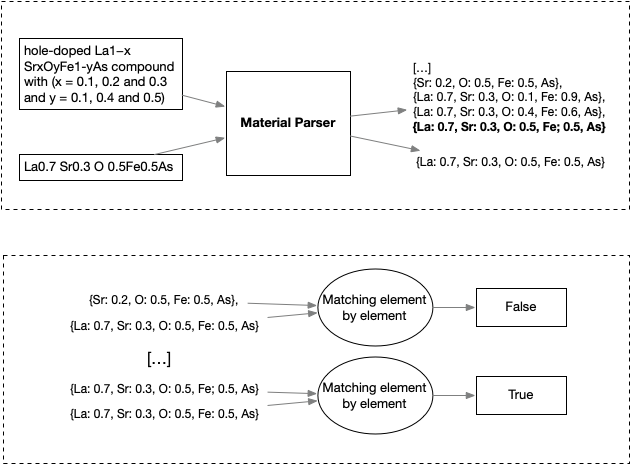
\includegraphics[width=1\textwidth]{figures/formula-matching-schema.png} 
  \caption{Two materials that appear to have a very different composition, are, in reality overlapping. (Top) Summary of the Material Parser. More information is available in~\cite{lfoppiano2023automatic}. (Bottom) The pairwise comparison of each chemical formula is performed element-by-element.  }
  \label{fig:formula-matching-schema}
\end{figure}

% Researchers frequently employ sets of variables as a convenient method to circumvent the explicit enumeration of nearly identical formulas, especially prevalent when discussing the substitution of one rare earth element with others, as exemplified by \texttt{RE x La 1-x O 7 with RE = Y, Pr, Sm, Eu, Gd and x = 0.1, 0.2}.


This approach extends strict matching and is activated only when the two input strings differ. In such instances, as depicted in Figure~\ref{fig:formula-matching-schema}, the material expressions slated for comparison undergo normalization to their formulas using a material parser developed in our prior work~\cite{lfoppiano2023automatic} (Figure~\ref{fig:formula-matching-schema} top). The material parser is adept at handling noisy material expressions, striving to parse them effectively. The anticipated output includes a structured representation with the chemical formula presented both as a raw string and as a dictionary, detailing elements and their respective quantities. Subsequently, these structures are compared element by element, as depicted in Figure~\ref{fig:formula-matching-schema} bottom.
The summarised evaluation scores described in Section~\ref{sec:results-ner-materials} are calculated using the formula matching. 

\subsection{Relation Extraction}
\label{sec:re}
The baseline is established by a rule-based algorithm from our previous work~\cite{lfoppiano2023automatic} which was evaluated with SuperMat and for which we report the aggregated result in Section~\ref{sec:re}. 

The prompts are designed by providing a list of entities and requesting the LLM to group them based on their relation. 
Differently from the NER task, the LLM is expected to reuse information that is passed in the prompt to compose the response: non-matching information is considered incorrect.
The summarised scores in Section~\ref{sec:results-re} are obtained with strict matching. 

The previous considerations remain applicable to both system and user prompts, with the task description reiterated within both the system and user prompts. 

\begin{lstlisting}[caption=System prompt for RE modified by emphasising the tasks]
You are a useful assistant, who knows about materials science, physics, chemistry and engineering.
You will be asked to compute relation extraction given a text and lists of entities. 
If you are not sure, don't try to make up your answer, just answer "None". 
\end{lstlisting}

We add specific rules to avoid the creation of invalid groups of relations: responses containing entities that are not supplied in the user prompt, or empty relation blocks. 

% \begin{lstlisting}[caption=Relation extraction using zero-shot prompting]
% Consider the following text in between triple quotes: 
% """
% {text}
% """

% Find the relations between lists of entities of different classes. 
% Apply strictly the following rules:  
%     - if the material is not specified, ignore the relation block,
%     - if tc is not specified in absolute values, ignore the relation block 
    
% Following are the lists of entities: 
% {entities}
% \end{lstlisting}

The prompt for few-shot learning was assembled by injecting two examples listed between two "--------" in the prompt for zero-shot learning:

\begin{lstlisting}[caption=Few-shot prompting for extracting relations from lists of entities]
Given a text between triple quotes and a list of entities, find the relations between entities of different classes: 
"""
{text}
"""

{entities}

--------
Example: 
The researchers of Mg have discovered that MgB2 is superconducting at 29 K at ambient pressure.

entities:
 materials: MgB2, Mg
 tcs: 29K
 pressure: ambient pressure
 
Result: 
 material: MgB2, 
 tc: 29K, 
 pressure: ambient pressure
 
--------
Apply strictly the following rules:  
    - if the material is not specified, ignore the relation block,
    - if tc is not specified in absolute values, ignore the relation block 
\end{lstlisting}

% The fine-tuned was implemented using the prompt used for the zero-shot prompting provided to a model that was fine-tuned using a partition of SuperMat (344 examples for training and 148 examples for testing) and evaluated with the rest (88 examples). One example represents a unique paragraph with multiple relations within.

The list of entities supplied to the Language Model (LLM) might be derived based on their order of appearance, creating a scenario where a model generating relations sequentially may achieve an inflated score that doesn't accurately reflect its relational inference capabilities. 
To address this, we offer two versions for each model and generation type: a \emph{non-shuffled} version, where entities are presented in their original order, and a \emph{shuffled} version, where entities are randomly rearranged before being introduced to the prompt.

\subsection{Consideration about the fine-tuning}

We fine-tuned the GPT-3.5-turbo model using the OpenAI platform which ingested train and test data, and generated a new model in a few hours. 
All models were trained using the default parameters selected by the OpenAI platform.

Table~\ref{tab:amount-data-fine-tuned} illustrates the dimension of each dataset. 
The fine-tuned model for properties extraction was trained using the "Quantities" dataset~\cite{foppiano2019quantities} because MeasEval did not contain enough examples for a consistent and unbiased evaluation. 

\begin{table}[htbp]
    \centering
    \label{tab:amount-data-fine-tuned}
    \caption{Amount of data used for training the fine-tuned models.}
    \begin{tabular}{lccc}
        Task & Dataset & \# Training & \# Test \\
        \toprule
        NER & SuperMat   & 1639 & 703 \\
        NER & Quantities & 485 & 208 \\
        RE  & SuperMat   & 344 & 148 \\
        \bottomrule
    \end{tabular}
\end{table}

The primary challenge encountered when employing a fine-tuned model was the necessity to achieve a valid, machine-readable JSON format. 
Therefore, we formatted the training data with an expected output in valid JSON format. 
However, the obtained fine-tuned model struggled to produce valid JSON in its output, leading us to hypothesise that this limitation might be attributed to a shortage of training examples. 
To address this, we modified our training data expected output from JSON to a pseudo format structured with spaces and break-lines, facilitating simpler handling by the model. The subsequent example illustrates the expected output for a RE task:

\begin{lstlisting}[caption=Example format of the expected answer for the RE task]
    material: mat1, tc: 22K, 
    material: mat2, tc: 24K, pressure: 2GPa
\end{lstlisting}

We followed the same approach for fine-tuning the model for the NER task: 

\begin{lstlisting}[caption=Example format of the expected answer for the NER task]
    materials: 
     - material1
     - material2
     - material3
\end{lstlisting}

Using this technique we could fine-tune a model that was still answering conversationally and then use the GPT-3.5-turbo base model to transform the response into JSON format. 

% \subsubsection{Open-source models}
% We tested the open-source models using an approximate implementation called Ollama, which can run small models on general hardware. 
% We tested Mistral-instruct-v0.1, Zehpyr-0.1-beta, MistralOpenOrca-

\section{Results and discussions}
\label{sec:results}
In this section, we present and discuss the aggregated results of our evaluations. The completed raw results are available in the Supplementary Material section. 

\subsection{NER on properties extraction}
\label{sec:results-ner-properties}

The assessment of property extraction was conducted utilising the MeasEval dataset, with the baseline established by grobid-quantities, achieving an approximately 85\% score using a holdout dataset created in tandem with the application. 
The evaluation of grobid-quantities~\cite{foppiano2019quantities} against MeasEval yielded a score of around 59\%. This disparity was anticipated, given the slightly divergent annotation strategies employed by the MeasEval developers compared to those used in the development of grobid-quantities (e.g. considerations such as approximate values and other proximity expressions were not taken into account). 

\begin{figure}[htbp]
  \centering
  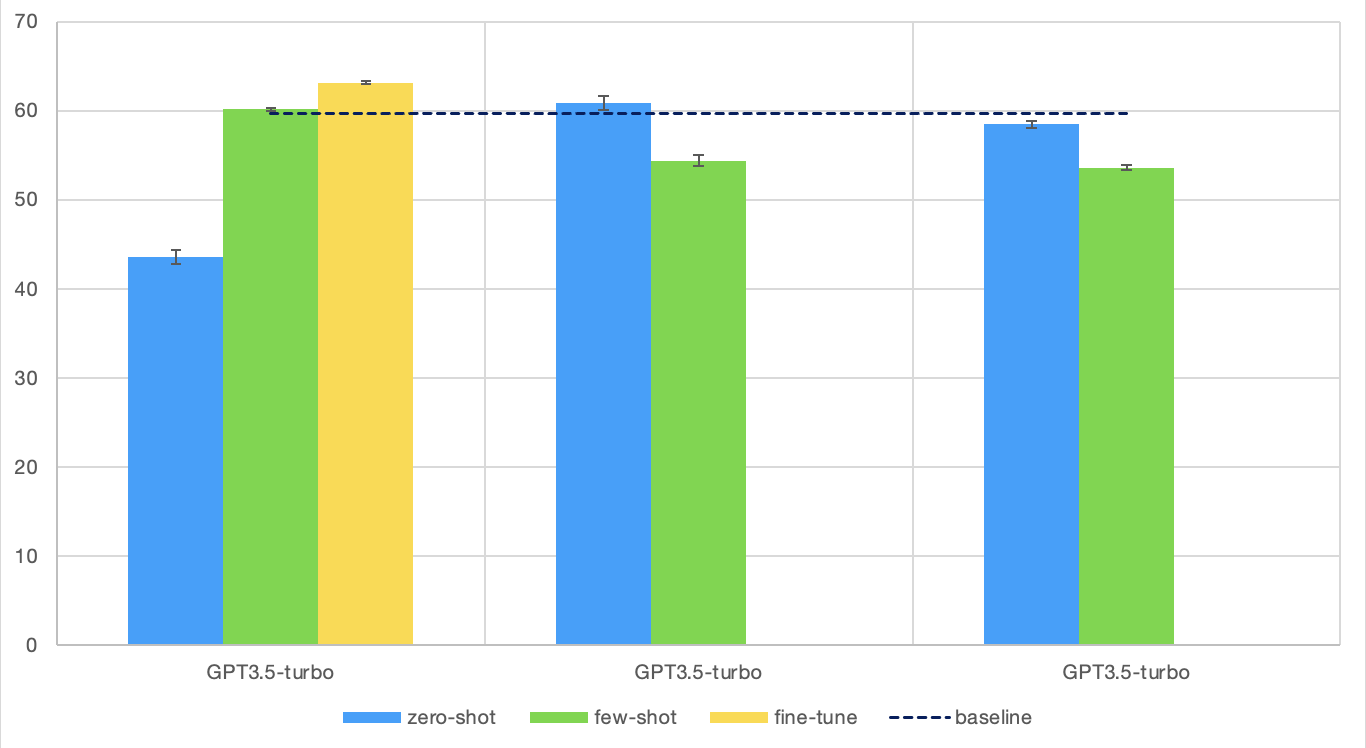
\includegraphics[width=0.78\textwidth]{figures/ner-measeval-all.png} 
  \caption{Comparison scores for properties extraction NER generation. The scores are the aggregations of the micro average F1 scores. The evaluation scores are calculated using soft matching with a threshold of 0.9 similarity. The error bars are calculated over the standard deviation of three independent runs.}
  \label{fig:ner-measeval-all}
\end{figure}

Unexpectedly, none of the models managed to outperform grobid-quantities in zero-shot learning, as depicted in Figure~\ref{fig:ner-measeval-all}. This outcome is surprising considering that a) the expression of properties lacks a specific domain constraint (aside from potential variations in frequency distribution), and b) quantities and measurements are likely prevalent in the extensive text corpus used to pre-train the OpenAI models.
In the realm of few-shot prompting (Figure~\ref{fig:ner-measeval-all}), a marginal improvement was observed only for GPT-4 and GPT-4-Turbo, resulting in an F1-score gain ranging around 2\%. 

However, this improvement is not substantial. 
We theorise that the hints provided to the Language Models (LLMs) may introduce bias, and when these hints are incorrect or incomplete, the LLMs struggle to guide the generation effectively, impacting the quality of the output results.
Significantly, the fine-tuned model (Figure~\ref{fig:ner-measeval-all}) appears to exhibit a slight enhancement compared to zero-shot, few-shot, and the baseline. Interestingly, in this specific instance where both the baseline and fine-tuned models are trained and evaluated on the same data, the LLM demonstrates an approximate 3\% increase in the F1-score.

\subsection{NER on materials expressions extraction}
\label{sec:results-ner-materials}
The evaluation of material expressions was performed using the validation partition of the SuperMat~\cite{lfoppiano2021supermat} dataset, composed of 32 articles.

\begin{figure}[htbp]
  \centering
  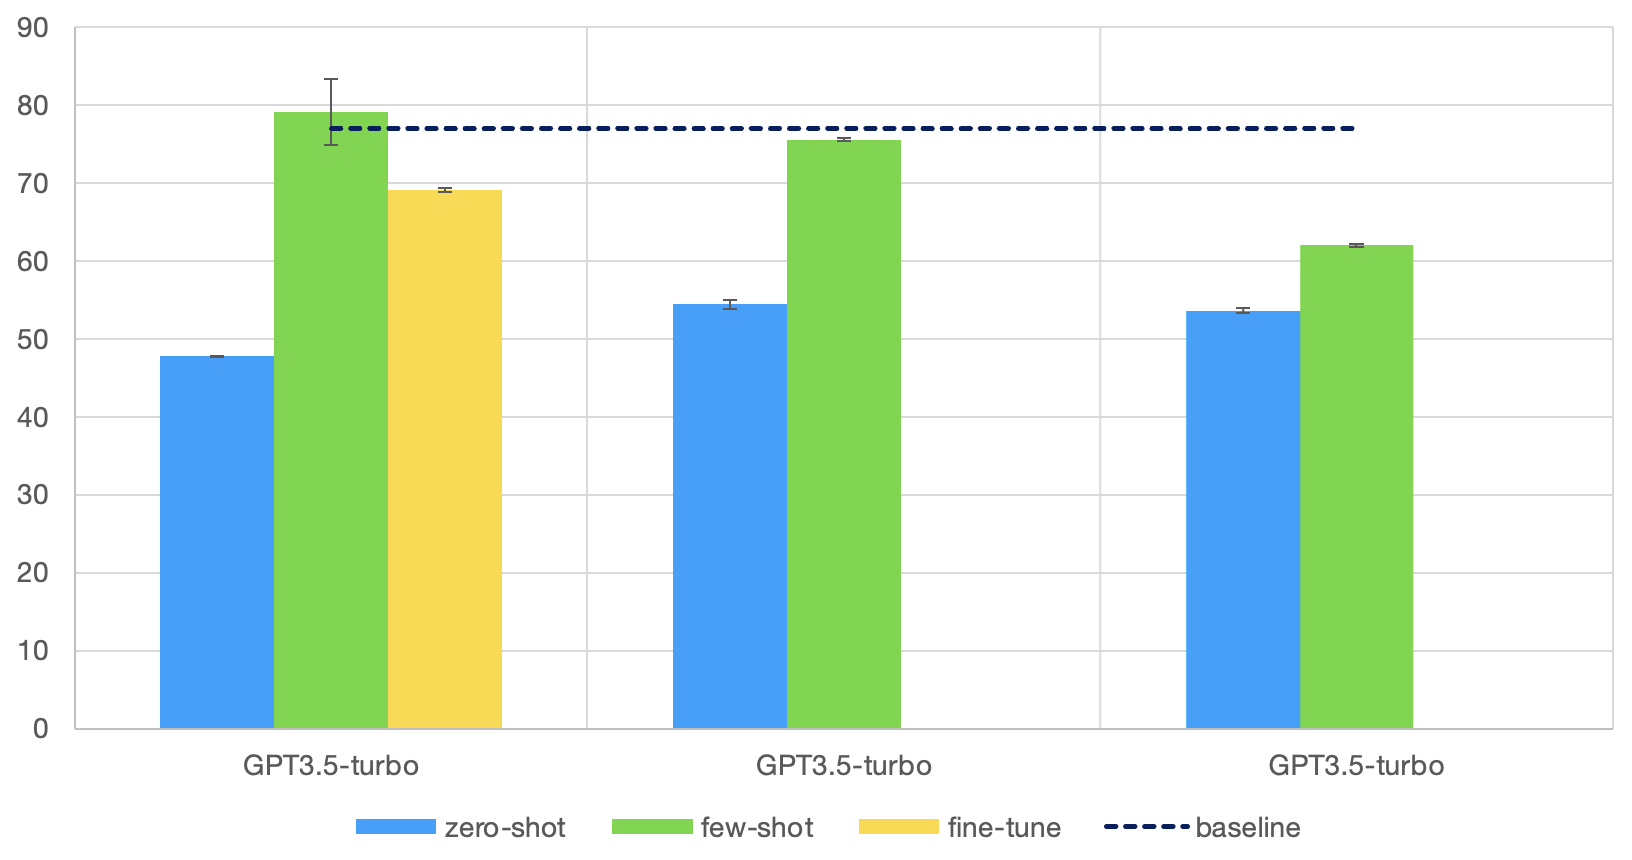
\includegraphics[width=0.8\textwidth]{figures/ner-supermat-all.png} 
  \caption{Comparison scores for the NER on materials extraction of the three models. The metrics are the aggregations of the micro average F1-scores, calculated using formula matching. The error bars are calculated over the standard deviation of three independent runs.}
  \label{fig:ner-materials-all}
\end{figure}

In zero-shot prompting (Figure~\ref{fig:ner-materials-all}), both GPT-4 and GPT-4-Turbo achieved comparable F1-scores, hovering around 50\%. Notably, all LLMs scored more than 10\% lower than the baseline~\cite{lfoppiano2023automatic}. This disparity is expected, given that material expressions may involve extensive sequences and encompass multiple pieces of information that are not easily conveyed in the prompt.
Few-shot prompting (Figure~\ref{fig:ner-materials-all}) yielded improved results, with GPT-3.5-turbo and GPT-4 slightly surpassing the baseline. 
The introduction of hints in the prompt indeed enhances performance, but, as previously discussed, it appears to strongly influence the LLMs, particularly to mitigate the impact of invalid hints that may be provided.
Equally unexpected, fine-tuning did not outperform few-shot prompting. This outcome suggests that the additional training did not significantly enhance the LLMs' ability to handle material expressions.

\subsection{Relation extraction}
\label{sec:results-re}

The evaluation of RE utilised the complete SuperMat dataset, with the results illustrated in Figure~\ref{fig:re-eval-all}, providing a comparison of the effects of shuffling across different models. 

\begin{figure}[htbp]
  \centering
  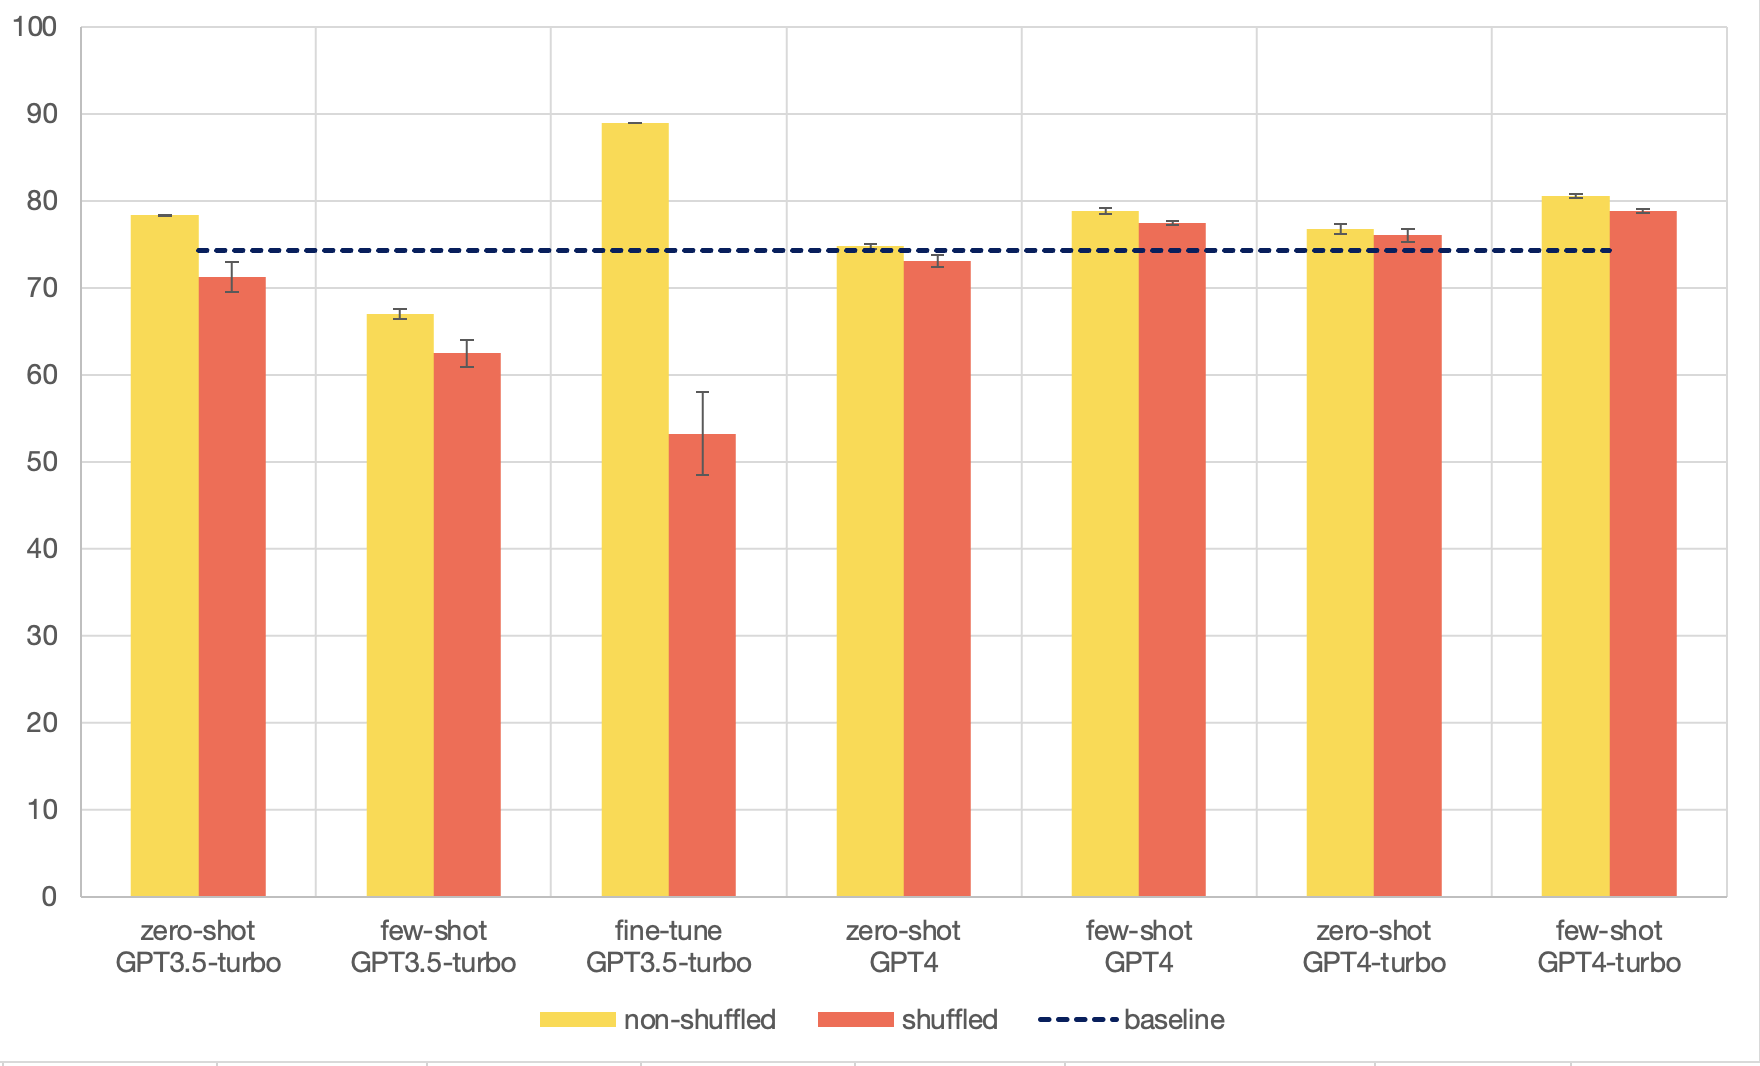
\includegraphics[width=0.8\textwidth]{figures/re-eval-all.png} 
  \caption{Comparison of the scores of the shuffled extraction using zero-shot, few-shot and fine-tuned of the three models for RE on materials and properties. The metrics are the aggregated micro average F1-scores calculated using strict matching. The error bars are calculated over the standard deviation of three independent runs.}
  \label{fig:re-eval-all}
\end{figure}

GPT-3.5-turbo demonstrates a significant difference between shuffled and non-shuffled approaches, suggesting a sequential connection of entities without specific contextual reasoning. 
Notably, the fine-tuned GPT-3.5-turbo model shows reduced flexibility, evident in a decreased F1 score during shuffled evaluation compared to the base model. 
In contrast, both GPT-4 and GPT-4-turbo exhibit minimal performance differences under shuffling conditions.

Figure~\ref{fig:re-eval-shuffled-all} specifically highlights the shuffled version of each model and extraction type. Except for GPT-3.5.5-turbo, few-shot prompting exhibits a substantial improvement compared to zero-shot prompting (Figure~\ref{fig:re-eval-shuffled-all}), achieved by incorporating additional examples in each prompt. 
Among the models, GPT-4-turbo attains the highest performance, reaching around an 80\% F1-score.

\begin{figure}[htbp]
  \centering
  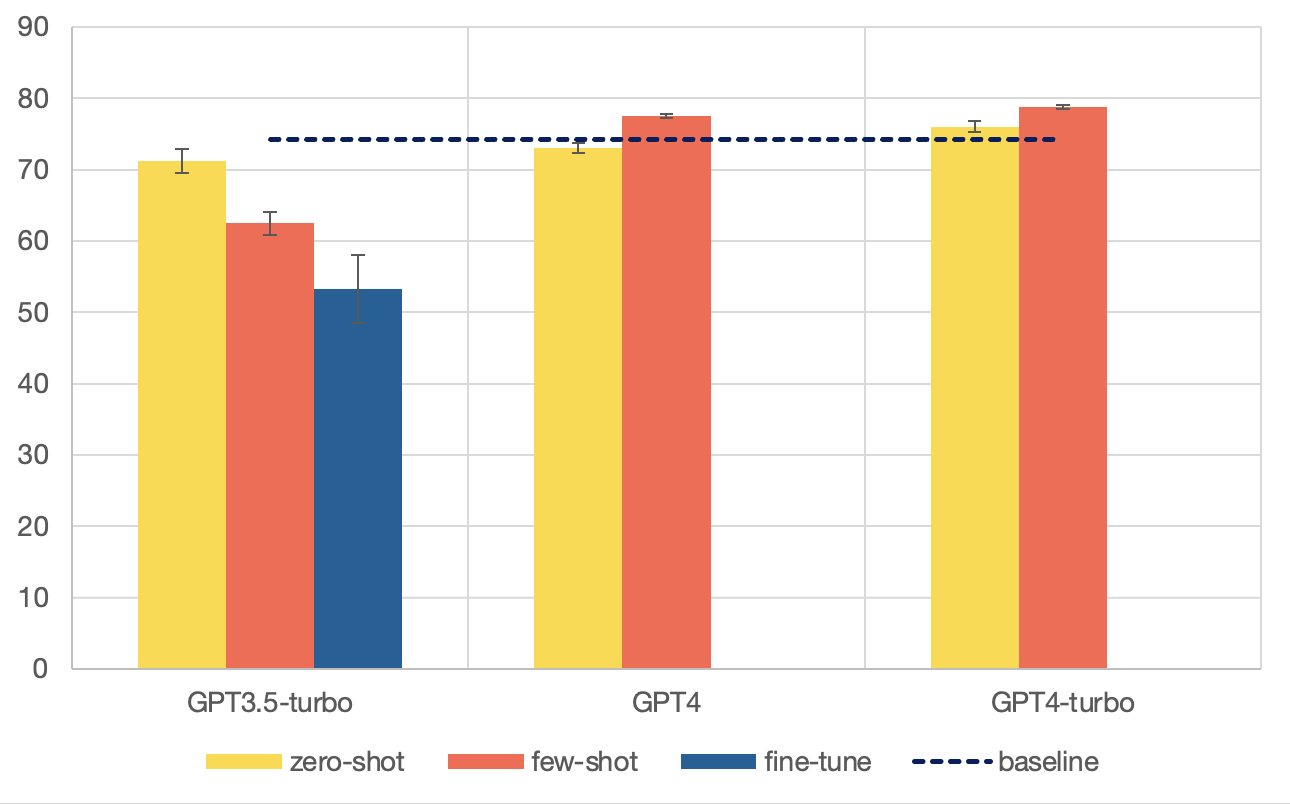
\includegraphics[width=0.8\textwidth]{figures/re-eval-shuffled-all.png} 
  \caption{Overview evaluation on the effect of shuffling the entities in RE on materials and properties. The metrics are the aggregated micro average F1-scores calculated using strict matching. The error bars are calculated over the standard deviation of three independent runs.}
  \label{fig:re-eval-shuffled-all}
\end{figure}

\section{Code availability}
This work is available at \url{https://github.com/lfoppiano/MatSci-LumEn}. The repository contains the scripts and the data used for extraction and evaluation. 
The code of the material parser used in the formula matching is available at \url{https://github.com/lfoppiano/material-parsers}, and the service API is accessible at \url{https://lfoppiano-material-parsers.hf.space}. 

\section{Conclusion}

When it comes to NER, LLMs appear to underperform significantly compared to SLMs in both material and property extraction (Q1)
This finding is particularly surprising considering properties since these expressions are not confined to a specific domain.

In material extraction, GPT3.5-turbo with fine-tuning failed to surpass the baseline, and the same holds for any model with few-shot prompting. 
For property extraction, GPT-4 and GPT-4 Turbo with zero-shot prompting perform on par with the baseline. GPT3.5-Turbo with few-shot and fine-tuning, on the other hand, outperform the baseline by a marginal increase in points.
Our results suggest that, for material expressions, small specialised models remain the most accurate choice.

The scenario improves for RE (Q2).
With two examples, few-shot prompting demonstrates a significant improvement over the baseline.
GPT-4 Turbo exhibits enhanced reasoning capabilities compared to GPT-4 and GPT-3.5 Turbo.
GPT-3.5 Turbo performs poorly in both zero-shot and few-shot prompting and shows a substantial score decrease when entities are shuffled, aligning with previous observations.
    
Fine-tuning, overall, does not appear to address all the challenges in both tasks and may struggle to learn to respond to a valid JSON format.

In conclusion, to answer Q2, GPT-4 and GPT-4-Turbo showcase effective reasoning capabilities for relating concepts and extracting relations accurately. 
GPT-4-Turbo, which costs one-third of GPT-4 remains a robust choice given its reasoning capabilities. 
However, for what concerns Q1, for the extraction of complex entities such as materials, we find that training small specialised models remains a more effective approach.


\section*{Acknowledgements}
Our warmest thanks to Patrice Lopez for his continuous support and inspiration with ideas, suggestions, and fruitful discussions.


\section*{Funding}
This work was partly supported by the MEXT Program: Data Creation and Utilization-Type Material Research and Development Project (Digital Transformation Initiative Center for Magnetic Materials) Grant Number JPMXP1122715503.


\section*{Notes on Contributors}
LF developed the scripts for extraction and evaluation and wrote the manuscript.
GL followed the LLM evaluation and technical side and financed the OpenAI bills. 
TA, GL and MI reviewed the article.
MI supervised the process and provided the budget. 



\bibliography{references}
\bibliographystyle{unsrt}

\clearpage

\appendix


\section{Full evaluation results}

\subsection{NER for properties extraction}

\subsubsection{Zero-shot prompting}
\begin{table}[htbp]
\small
  \centering
  \caption{Performance Metrics for GPT-3.5-turbo NER in properties extraction, zero-shot prompting. P: Precision, R: Recall, F1: harmonic average of P and R, Supp: Support, number of extracted entities.}
  \begin{tabular}{lccccc}
    \toprule
    \textbf{Run} & \textbf{Matching} & \textbf{P} & \textbf{R} & \textbf{F1} & \textbf{Supp} \\
    \midrule
    \multirow{2}{*}{Run1} & Soft matching & 42.73 & 14.49 & 21.64 & 564 \\
    & Sentence BERT & 45.39 & 15.39 & 22.99 & 564 \\
    \midrule
    \multirow{2}{*}{Run2} & Soft matching & 41.81 & 13.35 & 20.24 & 531 \\
    & Sentence BERT & 45.01 & 14.37 & 21.79 & 531 \\
    \midrule
    \multirow{2}{*}{Run3} & Soft matching & 42.86 & 14.61 & 21.79 & 567 \\
    & Sentence BERT & 45.86 & 15.63 & 23.32 & 567 \\
    \midrule
    \multicolumn{2}{l}{\textbf{Mean and Standard deviation of F1 score}} & & & & \\
    \midrule
    \textbf{Matching} & \textbf{Avg.} & $\sigma\textsuperscript{2}$ & & & \textbf{Avg. Supp}\\
    Soft matching & 21.22 & 0.85 & & & 554 \\
    Sentence BERT & 22.7 & 0.80 & & & \\
    \bottomrule
  \end{tabular}
\end{table}


\begin{table}[htbp]
\small
  \centering
  \caption{Performance Metrics for GPT-4 NER in properties extraction, zero-shot prompting. P: Precision, R: Recall, F1: harmonic average of P and R, Supp: Support, number of extracted entities.}
  \begin{tabular}{lccccc}
    \toprule
    \textbf{Run} & \textbf{Matching} & \textbf{P} & \textbf{R} & \textbf{F1} & \textbf{Supp} \\
    \midrule
    \multirow{2}{*}{Run1} & Soft matching & 61.43 & 56.70 & 58.97 & 1535 \\
    & Sentence BERT & 65.08 & 60.07 & 62.48 & 1535 \\
    \midrule
    \multirow{2}{*}{Run2} & Soft matching & 63.23 & 57.19 & 60.06 & 1504 \\
    & Sentence BERT & 66.42 & 60.07 & 63.09 & 1504 \\
    \midrule
    \multirow{2}{*}{Run3} & Soft matching & 62.83 & 56.52 & 59.51 & 1496 \\
    & Sentence BERT & 66.11 & 59.47 & 62.61 & 1496 \\
    \midrule
    \multicolumn{2}{l}{\textbf{Mean and Standard deviation of F1 score}} & & & & \\
    \midrule
    \textbf{Matching} & \textbf{Avg.} & $\sigma\textsuperscript{2}$ & & & \textbf{Avg. Supp}\\
    Soft matching & 59.51 & 0.54 & & & 1511 \\
    Sentence BERT & 62.72 & 0.32 & & & \\
    \bottomrule
  \end{tabular}
\end{table}


\begin{table}[htbp]
\small
  \centering
  \caption{Performance Metrics for GPT4-turbo NER in properties extraction, zero-shot prompting. P: Precision, R: Recall, F1: harmonic average of P and R, Supp: Support, number of extracted entities.}
  \begin{tabular}{lccccc}
    \toprule
    \textbf{Run} & \textbf{Matching} & \textbf{P} & \textbf{R} & \textbf{F1} & \textbf{Supp} \\
    \midrule
    \multirow{2}{*}{Run1} & Soft matching & 59.60 & 54.30 & 56.83 & 1515 \\
    & Sentence BERT & 62.90 & 57.31 & 59.97 & 1515 \\
    \midrule        
    \multirow{2}{*}{Run2} & Soft matching & 60.34 & 55.44 & 57.79 & 1528 \\
    & Sentence BERT & 63.87 & 58.69 & 61.17 & 1528 \\
    \midrule        
    \multirow{2}{*}{Run3} & Soft matching & 60.05 & 54.60 & 57.20 & 1512 \\    
    & Sentence BERT & 63.96 & 58.15 & 60.91 & 1512 \\
    \midrule
    \multicolumn{2}{l}{\textbf{Mean and Standard deviation of F1 score}} & & & & \\
    \midrule
    \textbf{Matching} & \textbf{Avg.} & $\sigma\textsuperscript{2}$ & & & \textbf{Avg. Supp}\\
    Soft matching & 57.27 & 0.48 & & & 1518 \\
    Sentence BERT & 60.68 & 0.63 & & & \\
    \bottomrule
  \end{tabular}
\end{table}

\clearpage
\subsubsection{Few-shot prompting }

\begin{table}[htbp]
\small
  \centering
  \caption{Performance Metrics for GPT-3.5-turbo NER in properties extraction, few-shot prompting. P: Precision, R: Recall, F1: harmonic average of P and R, Supp: Support, number of extracted entities.}
  \begin{tabular}{lccccc}
    \toprule
    \textbf{Run} & \textbf{Matching} & \textbf{P} & \textbf{R} & \textbf{F1} & \textbf{Supp} \\
    \midrule
    \multirow{2}{*}{Run1} & Soft matching & 60.98 & 57.79 & 59.34 & 1576 \\
    & Sentence BERT & 64.85 & 61.46 & 63.11 & 1576 \\    
    \midrule
    \multirow{2}{*}{Run2} & Soft matching & 60.99 & 57.73 & 59.31 & 1574 \\
    & Sentence BERT & 64.55 & 61.09 & 62.77 & 1574 \\
    \midrule
    \multirow{2}{*}{Run3} & Soft matching & 60.72 & 57.55 & 59.09 & 1576 \\
    & Sentence BERT & 64.28 & 60.91 & 62.55 & 1576 \\
    \midrule
    \multicolumn{2}{l}{\textbf{Mean and Standard deviation of F1 score}} & & & & \\
    \midrule
    \textbf{Matching} & \textbf{Avg.} & $\sigma\textsuperscript{2}$ & & & \textbf{Avg. Supp}\\
    Soft matching & 59.24 & 0.13 & & & 1575 \\
    Sentence BERT & 62.81 & 0.28 & & & \\
    \bottomrule
  \end{tabular}
\end{table}

\begin{table}[htbp]
\small
  \centering
  \caption{Performance Metrics for GPT-4 NER in properties extraction, few-shot prompting. P: Precision, R: Recall, F1: harmonic average of P and R, Supp: Support, number of extracted entities.}
  \begin{tabular}{lccccc}
    \toprule
    \textbf{Run} & \textbf{Matching} & \textbf{P} & \textbf{R} & \textbf{F1} & \textbf{Supp} \\
    \midrule
    \multirow{2}{*}{Run1} & Soft matching & 62.01 & 60.85 & 61.43 & 1632 \\
    & Sentence BERT & 65.56 & 64.34 & 64.95 & 1632 \\
    \midrule    
    \multirow{2}{*}{Run2} & Soft matching & 62.15 & 60.91 & 61.52 & 1630 \\
    & Sentence BERT & 65.52 & 64.22 & 64.86 & 1630 \\
    \midrule    
    \multirow{2}{*}{Run3} & Soft matching & 62.41 & 61.09 & 61.74 & 1628 \\
    & Sentence BERT & 65.6 & 64.22 & 64.9 & 1628 \\
    \midrule    
    \multicolumn{2}{l}{\textbf{Mean and Standard deviation of F1 score}} & & & & \\
    \midrule
    \textbf{Matching} & \textbf{Avg.} & $\sigma\textsuperscript{2}$ & & & \textbf{Avg. Supp}\\
    Soft matching & 61.56 & 0.16 & & & 1630 \\
    Sentence BERT & 64.9 & 0.04 & & & \\
    \bottomrule
  \end{tabular}
\end{table}

\begin{table}[htbp]
\small
  \centering
  \caption{Performance Metrics for GPT-4-turbo NER in properties extraction, few-shot prompting. P: Precision, R: Recall, F1: harmonic average of P and R, Supp: Support, number of extracted entities.}
  \begin{tabular}{lccccc}
    \toprule
    \textbf{Run} & \textbf{Matching} & \textbf{P} & \textbf{R} & \textbf{F1} & \textbf{Supp} \\
    \midrule
    \multirow{2}{*}{Run1} & Soft matching & 62.18 & 62 & 62.09 & 1652 \\
    & Sentence BERT & 65.8 & 65.6 & 65.7 & 1652 \\
    \midrule    
    \multirow{2}{*}{Run2} & Soft matching & 62.42 & 62.24 & 62.33 & 1658 \\
    & Sentence BERT & 66.1 & 65.9 & 66 & 1658 \\
    \midrule    
    \multirow{2}{*}{Run3} & Soft matching & 62.48 & 62.78 & 62.63 & 1671 \\
    & Sentence BERT & 65.95 & 66.27 & 66.11 & 1671 \\
    \midrule
    \multicolumn{2}{l}{\textbf{Mean and Standard deviation of F1 score}} & & & & \\
    \midrule
    \textbf{Matching} & \textbf{Avg.} & $\sigma\textsuperscript{2}$ & & & \textbf{Avg. Supp}\\
    Soft matching & 62.35 & 0.27 & & & 1660 \\
    Sentence BERT & 65.93 & 0.21 & & & \\
    \bottomrule
  \end{tabular}
\end{table}

\clearpage
\subsubsection{Fine-tuning}

\begin{table}[htbp]
\small
  \centering
  \caption{Performance Metrics for fine-tuned GPT-3.5-turbo NER in properties extraction. P: Precision, R: Recall, F1: harmonic average of P and R, Supp: Support, number of extracted entities.}
  \begin{tabular}{lccccc}
    \toprule
    \textbf{Run} & \textbf{Matching} & \textbf{P} & \textbf{R} & \textbf{F1} & \textbf{Supp} \\
    \midrule
    \multirow{2}{*}{Run1} & Soft matching & 60.76 & 58.57 & 59.64 & 1603 \\
    & Sentence BERT & 64.38 & 62.06 & 63.2 & 1603 \\
    \midrule
    \multirow{2}{*}{Run2} & Soft matching & 60.85 & 58.69 & 59.75 & 1604 \\
    & Sentence BERT & 64.4 & 62.12 & 63.24 & 1604 \\
    \midrule
    \multirow{2}{*}{Run3} & Soft matching & 60.49 & 58.45 & 59.45 & 1607 \\
    & Sentence BERT & 64.09 & 61.94 & 63 & 1607 \\
    \midrule
    \multicolumn{2}{l}{\textbf{Mean and Standard deviation of F1 score}} & & & & \\
    \midrule
    \textbf{Matching} & \textbf{Avg.} & $\sigma\textsuperscript{2}$ & & & \textbf{Avg. Supp}\\
    Soft matching & 59.61 & 0.15 & & & 1604 \\
    Sentence BERT & 63.14 & 0.12 & & & \\
    \bottomrule
  \end{tabular}
\end{table}

\clearpage
\subsection{NER for Materials extraction}

\subsubsection{Zero-shot}

\begin{table}[htbp]
\small
  \centering
  \caption{Performance Metrics for GPT3.5-turbo NER in materials extraction, zero-shot prompting. P: Precision, R: Recall, F1: harmonic average of P and R, Supp: Support, number of extracted entities.}
  \begin{tabular}{lccccc}
    \toprule
    \textbf{Run} & \textbf{Matching} & \textbf{P} & \textbf{R} & \textbf{F1} & \textbf{Supp} \\
    \midrule
    \multirow{2}{*}{Run1} & Sentence BERT & 37.34 & 22.58 & 28.14 & 1617 \\
    & Formula & 59.49 & 35.97 & 44.83 & 1617 \\
    \midrule
    \multirow{2}{*}{Run2} & Sentence BERT & 37.06 & 22.83 & 28.26 & 1641 \\
    & Formula & 59.21 & 36.48 & 45.15 & 1641 \\
    \midrule
    \multirow{2}{*}{Run3} & Sentence BERT & 37.45 & 22.07 & 27.77 & 1587 \\
    & Formula & 59.74 & 35.2 & 44.3 & 1587 \\
    \midrule
    \multicolumn{2}{l}{\textbf{Mean and Standard deviation of F1 score}} & & & & \\
    \midrule
    \textbf{Matching} & \textbf{Avg.} & $\sigma\textsuperscript{2}$ & & & \textbf{Avg. Supp}\\
    Sentence BERT & 28.05 & 0.25 & & & 1615 \\
    Formula & 44.76 & 0.42 & & & \\
    \bottomrule
  \end{tabular}
\end{table}



\begin{table}[htbp]
\small
  \centering
  \caption{Performance Metrics for GPT-4 NER in materials extraction, zero-shot prompting. P: Precision, R: Recall, F1: harmonic average of P and R, Supp: Support, number of extracted entities.}
  \begin{tabular}{lccccc}
    \toprule
    \textbf{Run} & \textbf{Matching} & \textbf{P} & \textbf{R} & \textbf{F1} & \textbf{Supp} \\
    \midrule
    \multirow{2}{*}{Run1} & Sentence BERT & 49.9 & 31.25 & 38.43 & 1103 \\
    & Formula & 66.4 & 41.58 & 51.14& 1103 \\
    \midrule
    \multirow{2}{*}{Run2} & Sentence BERT & 49.9 & 30.61 & 37.94 & 1097 \\
    & Formula & 66.94 & 41.07 & 50.91 & 1097 \\
    \midrule
    \multirow{2}{*}{Run3} & Sentence BERT & 49.59 & 30.74 & 37.95 & 1108 \\
    & Formula & 66.46 & 41.2 & 50.87 & 1108 \\
    \midrule
    \multicolumn{2}{l}{\textbf{Mean and Standard deviation of F1 score}} & & & & \\
    \midrule
    \textbf{Matching} & \textbf{Avg.} & $\sigma\textsuperscript{2}$ & & & \textbf{Avg. Supp}\\
    Sentence BERT & 38.10 & 0.28 & & & 1102 \\
    Formula & 50.97 & 0.14 & & & \\
    \bottomrule
  \end{tabular}
\end{table}

\begin{table}[htbp]
\small
  \centering
  \caption{Performance Metrics for GPT4-turbo NER in properties extraction, zero-shot prompting. P: Precision, R: Recall, F1: harmonic average of P and R, Supp: Support, number of extracted entities.}
  \begin{tabular}{lccccc}
    \toprule
    \textbf{Run} & \textbf{Matching} & \textbf{P} & \textbf{R} & \textbf{F1} & \textbf{Supp} \\
    \midrule
    \multirow{2}{*}{Run1} & Sentence BERT & 45.53 & 22.07 & 29.73 & 883 \\
    & Formula & 70.53 & 34.18 & 46.05 & 883 \\
    \midrule
    \multirow{2}{*}{Run2} & Sentence BERT & 46.67 & 22.32 & 30.2 & 873 \\
    & Formula & 70.67 & 33.8 & 45.73 & 873 \\
    \midrule
    \multirow{2}{*}{Run3} & Sentence BERT & 46.74 & 22.83 & 30.68 & 878 \\
    & Formula & 70.5 & 34.44 & 46.27 & 878 \\
    \midrule
    \multicolumn{2}{l}{\textbf{Mean and Standard deviation of F1 score}} & & & & \\
    \midrule
    \textbf{Matching} & \textbf{Avg.} & $\sigma\textsuperscript{2}$ & & & \textbf{Avg. Supp}\\
    Sentence BERT & 45.98 & 0.56 & & & 878 \\
    Formula & 53.60 & 0.30 & & & \\
    \bottomrule
  \end{tabular}
\end{table}


\clearpage
\subsubsection{Few-shot}

\begin{table}[htbp]
\small
  \centering
  \caption{Performance Metrics for GPT3.5-turbo NER in materials extraction, few-shot prompting. P: Precision, R: Recall, F1: harmonic average of P and R, Supp: Support, number of extracted entities.}
  \begin{tabular}{lccccc}
    \toprule
    \textbf{Run} & \textbf{Matching} & \textbf{P} & \textbf{R} & \textbf{F1} & \textbf{Supp} \\
    \midrule
    \multirow{2}{*}{Run1} & Sentence BERT & 71.58 & 69.39 & 70.47 & 1887 \\
    & Formula & 75.79 & 73.47 & 74.61 & 1887 \\
    \midrule
    \multirow{2}{*}{Run2} & Sentence BERT & 78.73 & 88.78 & 83.45 & 2495 \\
    & Formula & 78.39 & 88.39 & 83.09 & 2495 \\
    \midrule
    \multirow{2}{*}{Run3} & Sentence BERT & 78.85 & 88.9 & 83.57 & 2448 \\
    & Formula & 78.73 & 88.78 & 83.45 & 2448 \\
    \midrule
    \multicolumn{2}{l}{\textbf{Mean and Standard deviation of F1 score}} & & & & \\
    \midrule
    \textbf{Matching} & \textbf{Avg.} & $\sigma\textsuperscript{2}$ & & & \textbf{Avg. Supp}\\
    Sentence BERT & 79.16 & 7.5 & & & 2276 \\
    Formula & 80.38 & 4.82 & & & \\
    \bottomrule
  \end{tabular}
\end{table}


\begin{table}[htbp]
\small
  \centering
  \caption{Performance Metrics for GPT-4 NER in materials extraction, few-shot prompting. P: Precision, R: Recall, F1: harmonic average of P and R, Supp: Support, number of extracted entities.}
  \begin{tabular}{lccccc}
    \toprule
    \textbf{Run} & \textbf{Matching} & \textbf{P} & \textbf{R} & \textbf{F1} & \textbf{Supp} \\
    \midrule
    \multirow{2}{*}{Run1} & Sentence BERT & 75.87 & 75 & 75.43 & 1402 \\
    & Formula & 77.16 & 76.28 & 76.72 & 1412 \\
    \midrule
    \multirow{2}{*}{Run2} & Sentence BERT & 70.67 & 82.65 & 76.19 & 1402 \\
    & Formula & 70.99 & 83.04 & 76.54 & 1854 \\
    \midrule
    \multirow{2}{*}{Run3} & Sentence BERT & 70.99 & 83.04 & 76.54 & 1402 \\
    & Formula & 72.09 & 83.67 & 77.45 & 1826 \\
    \midrule
    \multicolumn{2}{l}{\textbf{Mean and Standard deviation of F1 score}} & & & & \\
    \midrule
    \textbf{Matching} & \textbf{Avg.} & $\sigma\textsuperscript{2}$ & & & \textbf{Avg. Supp}\\
    Sentence BERT & 76.35 & 1.02 & & & 1402 \\
    Formula & 76.90 & 0.48 & & & \\
    \bottomrule
  \end{tabular}
\end{table}


\begin{table}[htbp]
\small
  \centering
  \caption{Performance Metrics for GPT4-turbo NER in materials extraction, few-shot prompting. P: Precision, R: Recall, F1: harmonic average of P and R, Supp: Support, number of extracted entities.}
  \begin{tabular}{lccccc}
    \toprule
    \textbf{Run} & \textbf{Matching} & \textbf{P} & \textbf{R} & \textbf{F1} & \textbf{Supp} \\
    \midrule
    \multirow{2}{*}{Run1} & Sentence BERT & 54.78 & 59.95 & 57.25 & 1735 \\
    & Formula & 60.26 & 65.94 & 62.97 & 1735 \\
    \midrule
    \multirow{2}{*}{Run2} & Sentence BERT & 55.54 & 59.44 & 57.42 & 1707 \\
    & Formula & 60.91 & 65.18 & 62.97 & 1707 \\
    \midrule
    \multirow{2}{*}{Run3} & Sentence BERT & 55.81 & 60.08 & 57.86 & 1707 \\
    & Formula & 61.02 & 65.69 & 63.27 & 1707 \\
    \midrule
    \multicolumn{2}{l}{\textbf{Mean and Standard deviation of F1 score}} & & & & \\
    \midrule
    \textbf{Matching} & \textbf{Avg.} & $\sigma\textsuperscript{2}$ & & & \textbf{Avg. Supp}\\
    Sentence BERT & 57.51 & 0.31 & & & 1716 \\
    Formula & 63.07 & 0.17 & & & \\
    \bottomrule
  \end{tabular}
\end{table}

\clearpage
\subsubsection{Fine-tuning}

\begin{table}[htbp]
\small
  \centering
  \caption{Performance Metrics for the fine-tuned GPT3.5-turbo NER in materials extraction. P: Precision, R: Recall, F1: harmonic average of P and R, Supp: Support, number of extracted entities.}
  \begin{tabular}{lccccc}
    \toprule
    \textbf{Run} & \textbf{Matching} & \textbf{P} & \textbf{R} & \textbf{F1} & \textbf{Supp} \\
    \midrule
    \multirow{2}{*}{Run1} & Sentence BERT & 61.02 & 65.69 & 63.27 & 1429 \\
    & Formula & 61.02 & 65.69 & 63.27 & 1429 \\
    \midrule
    \multirow{2}{*}{Run2} & Sentence BERT & 72.24 & 67.73 & 69.91 & 1429 \\
    & Formula & 80.14 & 75.13 & 77.55 & 1429 \\
    \midrule
    \multirow{2}{*}{Run3} & Sentence BERT & 72.17 & 67.47 & 69.74 & 1432 \\
    & Formula & 80.08 & 74.87 & 77.39 & 1432 \\
    \midrule
    \multicolumn{2}{l}{\textbf{Mean and Standard deviation of F1 score}} & & & & \\
    \midrule
    \textbf{Matching} & \textbf{Avg.} & $\sigma\textsuperscript{2}$ & & & \textbf{Avg. Supp}\\
    Sentence BERT & 69.75 & 0.15 & & & 1430 \\
    Formula & 77.43 & 0.09 & & & \\
    \bottomrule
  \end{tabular}
\end{table}

\clearpage
\subsection{RE for Materials-Properties extraction}

\subsubsection{Zero-shot}

\begin{table}[htbp]
  \small
  \centering
  \caption{Performance Metrics for the GPT3.5-turbo model on RE in materials-properties extraction. In this run, entities are not shuffled when included in the prompt. P: Precision, R: Recall, F1: harmonic average of P and R, Supp: Support, number of extracted entities.}
  \begin{tabular}{lccccc}
    \toprule
    \textbf{Run} & \textbf{Matching} & \textbf{P} & \textbf{R} & \textbf{F1} & \textbf{Supp} \\
    \midrule
    \multirow{2}{*}{Run1} & Strict matching & 80.41 & 65.7 & 72.32 & 934 \\
    & Soft matching & 80.73 & 65.97 & 72.6 & 934 \\
    \midrule
    \multirow{2}{*}{Run2} & Strict matching & 80.41 & 54.59 & 65.03 & 776 \\
    & Soft matching & 80.8 & 54.86 & 65.35 & 776 \\
    \midrule
    \multirow{2}{*}{Run3} & Strict matching & 80.25 & 55.47 & 65.6 & 790 \\
    & Soft matching & 80.51 & 55.64 & 65.8 & 790 \\
    \midrule
    \multicolumn{2}{l}{\textbf{Mean and Standard deviation of F1 score}} & & & & \\
    \midrule
    \textbf{Matching} & \textbf{Avg.} & $\sigma\textsuperscript{2}$ & & & \textbf{Avg. Supp}\\
    Strict matching & 67.65 & 4.05 & & & 833 \\
    Soft matching & 67.91 & 4.06 & & & \\
    \bottomrule
  \end{tabular}
\end{table}


\begin{table}[htbp]
    \small
    \centering
    \caption{Performance Metrics for the GPT3.5-turbo model on RE in materials-properties extraction. In this run, entities are shuffled to make it more challenging for the LLM. P: Precision, R: Recall, F1: harmonic average of P and R, Supp: Support, number of extracted entities.}
    \begin{tabular}{lccccc}
        \toprule
        \textbf{Run} & \textbf{Matching} & \textbf{P} & \textbf{R} & \textbf{F1} & \textbf{Supp} \\
        \midrule
        \multirow{2}{*}{Run1} & Strict matching & 76.12 & 60.8 & 67.61 & 913 \\
        & Soft matching & 76.67 & 61.24 & 68.09 & 913 \\
        \midrule
        \multirow{2}{*}{Run2} & Strict matching & 72.08 & 48.56 & 58.02 & 770 \\
        & Soft matching & 73.12 & 49.26 & 58.86 & 770 \\
        \midrule
        \multirow{2}{*}{Run3} & Strict matching & 74.9 & 49.61 & 59.68 & 757 \\
        & Soft matching & 75.17 & 49.78 & 59.89 & 757 \\
        \midrule
        \multicolumn{2}{l}{\textbf{Mean and Standard deviation of F1 score}} & & & & \\
        \midrule
        \textbf{Matching} & \textbf{Avg.} & $\sigma\textsuperscript{2}$ & & & \textbf{Avg. Supp}\\
        Strict matching & 61.77 & 5.12 & & & 813 \\
        Soft matching & 62.28 & 5.05 & & \\
        \bottomrule
    \end{tabular}
\end{table}

%GPT4

\begin{table}[htbp]
    \small
    \centering
    \caption{Performance Metrics for the GPT-4 model on RE in materials-properties extraction. In this run, entities are not shuffled when added to the prompt. P: Precision, R: Recall, F1: harmonic average of P and R, Supp: Support, number of extracted entities.}
    \begin{tabular}{lccccc}
        \toprule
        \textbf{Run} & \textbf{Matching} & \textbf{P} & \textbf{R} & \textbf{F1} & \textbf{Supp} \\
        \midrule
        \multirow{2}{*}{Run1} & Strict matching & 76.87 & 66.58 & 71.35 & 990 \\
        & Soft matching & 77.47 & 67.1 & 71.92 & 990 \\
        \midrule
        \multirow{2}{*}{Run2} & Strict matching & 76.4 & 67.98 & 71.94 & 1017 \\
        & Soft matching & 76.5 & 68.07 & 72.04 & 1017 \\
        \midrule
        \multirow{2}{*}{Run3} & Strict matching & 76.8 & 68.07 & 72.17 & 1013 \\
        & Soft matching & 76.9 & 68.15 & 72.26 & 1013 \\
        \midrule
        \multicolumn{2}{l}{\textbf{Mean and Standard deviation of F1 score}} & & & & \\
        \midrule
        \textbf{Matching} & \textbf{Avg.} & $\sigma\textsuperscript{2}$ & & & \textbf{Avg. Supp}\\
        Strict matching & 71.82 & 0.42 & & & 1006 \\
        Soft matching   & 72.07 & 0.17 & & \\
        \bottomrule
    \end{tabular}
\end{table}


\begin{table}[htbp]
    \small
    \centering
    \caption{Performance Metrics for the GPT4 model on RE in materials-properties extraction. In this run, entities are shuffled to make it more challenging for the LLM. P: Precision, R: Recall, F1: harmonic average of P and R, Supp: Support, number of extracted entities.}
    \begin{tabular}{lccccc}
        \toprule
        \textbf{Run} & \textbf{Matching} & \textbf{P} & \textbf{R} & \textbf{F1} & \textbf{Supp} \\
        \midrule
        \multirow{2}{*}{Run1} & Strict matching & 75.86 & 65.97 & 70.57 & 994 \\
        & Soft matching & 76.16 & 66.23 & 70.85 & 994 \\
        \midrule
        \multirow{2}{*}{Run2} & Strict matching & 74.06 & 65.44 & 69.48 & 1010 \\
        & Soft matching & 74.06 & 65.44 & 69.48 & 1010 \\
        \midrule
        \multirow{2}{*}{Run3} & Strict matching & 75.37 & 66.4 & 70.6 & 1007 \\
        & Soft matching & 75.57 & 66.58 & 70.79 & 1007 \\
        \midrule
        \multicolumn{2}{l}{\textbf{Mean and Standard deviation of F1 score}} & & & & \\
        \midrule
        \textbf{Matching} & \textbf{Avg.} & $\sigma\textsuperscript{2}$ & & & \textbf{Avg. Supp}\\
        Strict matching & 70.21 & 0.63 & & & 1003 \\
        Soft matching   & 70.37 & 0.77 & & \\
        \bottomrule
    \end{tabular}
\end{table}


% GPT4-turbo
\begin{table}[htbp]
    \small
    \centering
    \caption{Performance Metrics for the GPT4-turbo model on RE in materials-properties extraction. In this run, entities are not shuffled when added to the prompt. P: Precision, R: Recall, F1: harmonic average of P and R, Supp: Support, number of extracted entities.}
    \begin{tabular}{lccccc}
        \toprule
        \textbf{Run} & \textbf{Matching} & \textbf{P} & \textbf{R} & \textbf{F1} & \textbf{Supp} \\
        \midrule
        \multirow{2}{*}{Run1} & Strict matching & 79.8 & 69.12 & 74.07 & 990 \\
        & Soft matching & 80.61 & 69.82 & 74.82 & 990 \\
        \midrule
        \multirow{2}{*}{Run2} & Strict matching & 80.22 & 69.2 & 74.31 & 986 \\
        & Soft matching & 81.03 & 69.9 & 75.06 & 986 \\
        \midrule
        \multirow{2}{*}{Run3} & Strict matching & 78.87 & 73.65 & 76.17 & 989 \\
        & Soft matching & 79.88 & 69.12 & 74.11 & 989 \\
        \midrule
        \multicolumn{2}{l}{\textbf{Mean and Standard deviation of F1 score}} & & & & \\
        \midrule
        \textbf{Matching} & \textbf{Avg.} & $\sigma\textsuperscript{2}$ & & & \textbf{Avg. Supp}\\
        Strict matching & 73.85	& 0.60 & & & 988 \\
        Soft matching & 74.66 & 0.49 & & \\
        \bottomrule
    \end{tabular}
\end{table}

\begin{table}[htbp]
    \small
    \centering
    \caption{Performance Metrics for the GPT4-turbo model on RE in materials-properties extraction. In this run, entities are shuffled to make it more challenging for the LLM. P: Precision, R: Recall, F1: harmonic average of P and R, Supp: Support, number of extracted entities.}
    \begin{tabular}{lccccc}
        \toprule
        \textbf{Run} & \textbf{Matching} & \textbf{P} & \textbf{R} & \textbf{F1} & \textbf{Supp} \\
        \midrule
        \multirow{2}{*}{Run1} & Strict matching & 80.04 & 67.37 & 73.16 & 962 \\
        & Soft matching & 80.98 & 68.15 & 74.01 & 962 \\
        \midrule
        \multirow{2}{*}{Run2} & Strict matching & 80.71 & 67.72 & 73.64 & 959 \\
        & Soft matching & 81.44 & 68.33 & 74.31 & 959 \\
        \midrule
        \multirow{2}{*}{Run3} & Strict matching & 79.27 & 66.58 & 72.37 & 960 \\
        & Soft matching & 80.21 & 66.58 & 72.37 & 960 \\
        \midrule
        \multicolumn{2}{l}{\textbf{Mean and Standard deviation of F1 score}} & & & & \\
        \midrule
        \textbf{Matching} & \textbf{Avg.} & $\sigma\textsuperscript{2}$ & & & \\
        Strict matching & 76.05 & 0.74 & & & 960 \\
        Soft matching & 76.87 & 0.64 & & & \\
        \bottomrule
    \end{tabular}
\end{table}


\clearpage
\subsubsection{Few-shot}

% gpt3.5-turbo few shot not shuffled 

\begin{table}[htbp]
    \small
    \centering
    \caption{Performance Metrics for the GPT3.5-turbo model on RE in materials-properties extraction. In this run, entities are shuffled to make it more challenging for the LLM. P: Precision, R: Recall, F1: harmonic average of P and R, Supp: Support, number of extracted entities.}
    \begin{tabular}{lccccc}
        \toprule
        \textbf{Run} & \textbf{Matching} & \textbf{P} & \textbf{R} & \textbf{F1} & \textbf{Supp} \\
        \midrule
        \multirow{2}{*}{Run1} & Strict matching & 67.97 & 50.31 & 57.82 & 846 \\
        & Soft matching & 69.27 & 51.27 & 58.92 & 846 \\
        \midrule
        \multirow{2}{*}{Run2} & Strict matching & 68.2 & 50.48 & 58.02 & 846 \\
        & Soft matching & 69.5 & 51.44 & 59.13 & 846 \\
        \midrule
        \multirow{2}{*}{Run3} & Strict matching & 69.23 & 50.39 & 58.33 & 832 \\
        & Soft matching & 71.18 & 51.09 & 59.14 & 832 \\
        \midrule
        \multicolumn{2}{l}{\textbf{Mean and Standard deviation of F1 score}} & & & & \\
        \midrule
        \textbf{Matching} & \textbf{Avg.} & $\sigma\textsuperscript{2}$ & & & \textbf{Avg. Supp}\\
        Strict matching & 58.05 & 0.25 & & & 841 \\
        Soft matching & 59.06 & 0.12 & & & \\
        \bottomrule
    \end{tabular}
\end{table}


% gpt3.5-turbo few shot shuffled 
\begin{table}[htbp]
    \small
    \centering
    \caption{Performance Metrics for the GPT3.5-turbo model on RE in materials-properties extraction. In this run, entities are shuffled to make it more challenging for the LLM. P: Precision, R: Recall, F1: harmonic average of P and R, Supp: Support, number of extracted entities.}
    \begin{tabular}{lccccc}
        \toprule
        \textbf{Run} & \textbf{Matching} & \textbf{P} & \textbf{R} & \textbf{F1} & \textbf{Supp} \\
        \midrule
        \multirow{2}{*}{Run1} & Strict matching & 63.97 & 47.68 & 54.64 & 852 \\
        & Soft matching & 66.08 & 49.26 & 56.44 & 852 \\
        \midrule
        \multirow{2}{*}{Run2} & Strict matching & 66.02 & 47.59 & 55.31 & 824 \\
        & Soft matching & 67.23 & 48.47 & 56.33 & 824 \\
        \midrule
        \multirow{2}{*}{Run3} & Strict matching & 62.24 & 45.14 & 52.33 & 829 \\
        & Soft matching & 63.93 & 46.37 & 53.75 & 829 \\
        \midrule
        \multicolumn{2}{l}{\textbf{Mean and Standard deviation of F1 score}} & & & & \\
        \midrule
        \textbf{Matching} & \textbf{Avg.} & $\sigma\textsuperscript{2}$ & & & \textbf{Avg. Supp}\\
        Strict matching & 54.09 & 1.56 & & & 835 \\
        Soft matching   & 55.50 & 1.52 & & \\
        \bottomrule
    \end{tabular}
\end{table}

% GPT4 few shot not shuffled 
\begin{table}[htbp]
    \small
    \centering
    \caption{Performance Metrics for the GPT4 model on RE in materials-properties extraction. In this run, entities are not shuffled when they are added to the prompt. P: Precision, R: Recall, F1: harmonic average of P and R, Supp: Support, number of extracted entities.}
    \begin{tabular}{lccccc}
        \toprule
        \textbf{Run} & \textbf{Matching} & \textbf{P} & \textbf{R} & \textbf{F1} & \textbf{Supp} \\
        \midrule
        \multirow{2}{*}{Run1} & Strict matching & 80.57 & 71.83 & 75.95 & 1019 \\
        & Soft matching & 80.57 & 71.83 & 75.95 & 1019 \\
        \midrule
        \multirow{2}{*}{Run2} & Strict matching & 81.29 & 72.62 & 76.71 & 1021 \\
        & Soft matching & 81.39 & 72.7  & 76.8 & 1021 \\
        \midrule
        \multirow{2}{*}{Run3} & Strict matching & 80.9 & 72.27 & 76.34 & 1021 \\
        & Soft matching & 80.9 & 72.27 & 76.34 & 1021 \\
        \midrule
        \multicolumn{2}{l}{\textbf{Mean and Standard deviation of F1 score}} & & & & \\
        \midrule
        \textbf{Matching} & \textbf{Avg.} & $\sigma\textsuperscript{2}$ & & & \textbf{Avg. Supp}\\
        Strict matching & 76.33 & 0.38 & & & 1020 \\
        Soft matching & 76.36 & 0.42 & & \\
        \bottomrule
    \end{tabular}
\end{table}

% gpt4 few-shot shuffled 

\begin{table}[htbp]
    \small
    \centering
    \caption{Performance Metrics for the GPT4 model on RE in materials-properties extraction. In this run, entities are shuffled to make the task more challenging for the LLM. P: Precision, R: Recall, F1: harmonic average of P and R, Supp: Support, number of extracted entities.}
    \begin{tabular}{lccccc}
        \toprule
        \textbf{Run} & \textbf{Matching} & \textbf{P} & \textbf{R} & \textbf{F1} & \textbf{Supp} \\
        \midrule
        \multirow{2}{*}{Run1} & Strict matching & 80.57 & 70.17 & 74.5 & 1010 \\
        & Soft matching & 80.57 & 70.25 & 74.59 & 1010 \\
        \midrule
        \multirow{2}{*}{Run2} & Strict matching & 81.29 & 70.87 & 75.03 & 1016 \\
        & Soft matching & 81.39 & 71.13 & 75.31 & 1016 \\
        \midrule
        \multirow{2}{*}{Run3} & Strict matching & 80.9 & 70.6 & 75.07 & 1007 \\
        & Soft matching & 80.9 & 70.6 & 75.07 & 1007 \\
        \midrule
        \multicolumn{2}{l}{\textbf{Mean and Standard deviation of F1 score}} & & & & \\
        \midrule
        \textbf{Matching} & \textbf{Avg.} & $\sigma\textsuperscript{2}$ & & & \textbf{Avg. Supp}\\
        Strict matching & 74.86 & 0.31 & & & 1011 \\
        Soft matching & 74.99 & 0.36 & & \\
        \bottomrule
    \end{tabular}
\end{table}

% GPT4-turbo not shuffled 

\begin{table}[htbp]
    \small
    \centering
    \caption{Performance Metrics for the GPT4-turbo model on RE in materials-properties extraction. In this run, entities are not shuffled when they are added to the prompt. P: Precision, R: Recall, F1: harmonic average of P and R, Supp: Support, number of extracted entities.}
    \begin{tabular}{lccccc}
        \toprule
        \textbf{Run} & \textbf{Matching} & \textbf{P} & \textbf{R} & \textbf{F1} & \textbf{Supp}\\
        \midrule
        \multirow{2}{*}{Run1} & Strict matching & 83.44 & 70.08 & 76.18 & 960 \\
        & Soft matching & 84.69 & 71.13 & 77.32 & 960 \\
        \midrule
        \multirow{2}{*}{Run2} & Strict matching & 84.1 & 70.34 & 76.61 & 956 \\
        & Soft matching & 85.46 & 71.48 & 77.85 & 956 \\
        \midrule
        \multirow{2}{*}{Run3} & Strict matching & 84.01 & 70.34 & 76.57 & 957 \\
        & Soft matching & 85.37 & 71.48 & 77.81 & 957 \\
        \midrule
        \multicolumn{2}{l}{\textbf{Mean and Standard deviation of F-Score}} & & & & \\
        \midrule
        \textbf{Matching} & \textbf{Avg.} & $\sigma\textsuperscript{2}$ & & & \textbf{Avg. Supp}\\
        Strict matching & 76.45 & 0.23 & & & 957 \\
        Soft matching & 77.66 & 0.29 & & \\
        \bottomrule
    \end{tabular}
\end{table}

% GPT4-turbo  shuffled 

\begin{table}[htbp]
    \small
    \centering
    \caption{Performance Metrics for the GPT4-turbo model on RE in materials-properties extraction. In this run, entities are shuffled to make the task more challenging for the LLM. P: Precision, R: Recall, F1: harmonic average of P and R, Supp: Support, number of extracted entities.}
    \begin{tabular}{lccccc}
        \toprule
        \textbf{Run} & \textbf{Matching} & \textbf{P} & \textbf{R} & \textbf{F1} & \textbf{Supp} \\
        \midrule
        \multirow{2}{*}{Run1} & Strict matching & 82.01 & 67.02 & 73.76 & 934 \\
        & Soft matching & 83.51 & 68.24 & 75.11 & 934 \\
        \midrule
        \multirow{2}{*}{Run2} & Strict matching & 84.11 & 69.47 & 76.09 & 944 \\
        & Soft matching & 85.49 & 70.6 & 77.34 & 944 \\
        \midrule
        \multirow{2}{*}{Run3} & Strict matching & 82.31 & 67.98 & 74.46 & 944 \\
        & Soft matching & 84.32 & 69.64 & 76.28 & 944 \\
        \midrule
        \multicolumn{2}{l}{\textbf{Mean and Standard deviation of F-Score}} & & & & \\
        \midrule
        \textbf{Matching} & \textbf{Avg.} & $\sigma\textsuperscript{2}$ & & & \textbf{Avg. Supp}\\
        Strict matching & 74.77 & 1.19 & & & 940 \\
        Soft matching & 76.24 & 1.11 & & \\
        \bottomrule
    \end{tabular}
\end{table}

\clearpage
\subsubsection{Fine-tuning}

\begin{table}[htbp]
    \small
    \centering
    \caption{Performance Metrics for the GPT3.5-turbo model fine-tuned using the strategy "FT.base" on RE in materials-properties extraction. In this run, entities are not shuffled when included in the prompt. P: Precision, R: Recall, F1: harmonic average of P and R, Supp: Support, number of extracted entities.}
    \begin{tabular}{lccccc}
        \toprule
        \textbf{Run} & \textbf{Matching} & \textbf{P} & \textbf{R} & \textbf{F1} & \textbf{Supp} \\
        \midrule
        \multirow{2}{*}{Run1} & Strict matching & 91.06 & 80.00 & 85.17 & 123 \\
        & Soft matching & 93.50 & 82.14 & 87.45 & 123 \\
        \midrule
        \multirow{2}{*}{Run2} & Strict matching & 91.06 & 80.00 & 85.17 & 123 \\
        & Soft matching & 93.50 & 82.14 & 87.45 & 123 \\
        \midrule
        \multirow{2}{*}{Run3} & Strict matching & 91.06 & 80.00 & 85.17 & 123 \\
        & Soft matching & 93.50 & 82.14 & 87.45 & 123 \\
        \midrule
        \multicolumn{2}{l}{\textbf{Mean and Standard deviation of F1 score}} & & & & \\
        \midrule
        \textbf{Matching} & \textbf{Avg.} & $\sigma\textsuperscript{2}$ & & & \textbf{Avg. Supp}\\
        Strict matching & 85.17 & 0 &  & &  123 \\
        Soft matching & 87.45 & 0 & \\
        \bottomrule
    \end{tabular}
\end{table}


\begin{table}[htbp]
    \small
    \centering
    \caption{Performance Metrics for the GPT3.5-turbo model fine-tuned using the strategy "FT.base" on RE in materials-properties extraction. In this run, entities are shuffled to make it more challenging for the LLM. P: Precision, R: Recall, F1: harmonic average of P and R, Supp: Support, number of extracted entities.}
    \begin{tabular}{lccccc}
        \toprule
        \textbf{Run} & \textbf{Matching} & \textbf{P} & \textbf{R} & \textbf{F1} & \textbf{Supp} \\
        \midrule
        \multirow{2}{*}{Run1} & Strict matching & 92.68 & 81.43 & 86.69 & 123 \\
        & Soft matching & 95.12 & 83.57 & 88.97 & 123 \\
        \midrule
        \multirow{2}{*}{Run2} & Strict matching & 91.8 & 80 & 85.5 & 122 \\
        & Soft matching & 94.26 & 82.14 & 87.79 & 122 \\
        \midrule
        \multirow{2}{*}{Run3} & Strict matching & 91.06 & 80 & 85.17 & 123 \\
        & Soft matching & 93.5 & 82.14 & 87.45 & 123 \\
        \midrule
        \multicolumn{2}{l}{\textbf{Mean and Standard deviation of F1 score}} & & & & \\
        \midrule
        \textbf{Matching} & \textbf{Avg.} & $\sigma\textsuperscript{2}$ & & &  \textbf{Avg. Supp}\\
        Strict matching & 85.78 & 0.79 & & & 123 \\
        Soft matching & 88.07 & 0.79 & & \\
        \bottomrule
    \end{tabular}
\end{table}


\begin{table}[htbp]
    \small
    \centering
    \caption{Performance Metrics for the GPT3.5-turbo model fine-tuned using the strategy "FT.document\_order" on RE in materials-properties extraction. In this run, entities are not shuffled when included in the prompt. P: Precision, R: Recall, F1: harmonic average of P and R, Supp: Support, number of extracted entities.}
    \begin{tabular}{lccccc}
        \toprule
        \textbf{Run} & \textbf{Matching} & \textbf{P} & \textbf{R} & \textbf{F1} & \textbf{Supp} \\
        \midrule
        \multirow{2}{*}{Run1}   & Strict matching   & 88.98 & 80.71 & 84.64 & 127 \\
                                & Soft matching     & 91.34 & 82.86 & 86.89 & 127 \\
        \midrule
        \multirow{2}{*}{Run2}   & Strict matching   & 88.98 & 80.71 & 84.64 & 127 \\
                                & Soft matching     & 91.34 & 82.86 & 86.89 & 127 \\
        \midrule
        \multirow{2}{*}{Run3}   & Strict matching   & 88.98 & 80.71 & 84.64 & 127 \\
                                & Soft matching     & 91.34 & 82.86 & 86.89 & 127 \\
        \midrule
        \multicolumn{2}{l}{\textbf{Mean and Standard deviation of F1 score}} & & & & \\
        \midrule
        \textbf{Matching} & \textbf{Avg.} & $\sigma\textsuperscript{2}$ & & & \textbf{Avg. Supp}\\
        Strict matching & 84.64 & 0 &  & &  123 \\
        Soft matching   & 86.89 & 0 & \\
        \bottomrule
    \end{tabular}
\end{table}

\begin{table}[htbp]
    \small
    \centering
    \caption{Performance Metrics for the GPT3.5-turbo model fine-tuned using the strategy "FT.document\_order" on RE in materials-properties extraction. In this run, entities are shuffled to make it more challenging for the LLM. P: Precision, R: Recall, F1: harmonic average of P and R, Supp: Support, number of extracted entities.}
    \begin{tabular}{lccccc}
        \toprule
        \textbf{Run} & \textbf{Matching} & \textbf{P} & \textbf{R} & \textbf{F1} & \textbf{Supp} \\
        \midrule
        \multirow{2}{*}{Run1}   & Strict matching   & 47.73 & 45 & 46.32 & 132 \\
                                & Soft matching     & 48.48 & 45.71  & 47.06 & 132 \\
        \midrule
        \multirow{2}{*}{Run2}   & Strict matching   & 55.73 & 52.14  & 53.87 & 131 \\
                                & Soft matching     & 55.73 & 52.14  & 53.87 & 131 \\
        \midrule
        \multirow{2}{*}{Run3}   & Strict matching   & 57.72 & 50.71  & 53.99 & 123 \\
                                & Soft matching     & 57.72 & 50.71  & 53.99 & 123 \\
        \midrule
        \multicolumn{2}{l}{\textbf{Mean and Standard deviation of F1 score}} & & & & \\
        \midrule
        \textbf{Matching} & \textbf{Avg.} & $\sigma\textsuperscript{2}$ & & &  \textbf{Avg. Supp}\\
        Strict matching & 51.39 & 4.39 & & & 123 \\
        Soft matching & 51.64 & 3.96 & & \\
        \bottomrule
    \end{tabular}
\end{table}


\begin{table}[htbp]
    \small
    \centering
    \caption{Performance Metrics for the GPT3.5-turbo model fine-tuned using the strategy "FT.augmented" on RE in materials-properties extraction. In this run, entities are not shuffled when included in the prompt. P: Precision, R: Recall, F1: harmonic average of P and R, Supp: Support, number of extracted entities.}
    \begin{tabular}{lccccc}
        \toprule
        \textbf{Run} & \textbf{Matching} & \textbf{P} & \textbf{R} & \textbf{F1} & \textbf{Supp} \\
        \midrule
        \multirow{2}{*}{Run1}   & Strict matching   & 89.6 & 80 & 84.53 & 125 \\
                                & Soft matching     & 92 & 82.14 & 86.79 & 125 \\
        \midrule
        \multirow{2}{*}{Run2}   & Strict matching   & 89.6 & 80 & 84.53 & 125 \\
                                & Soft matching     & 92 & 82.14 & 86.79 & 125 \\
        \midrule
        \multirow{2}{*}{Run3}   & Strict matching   & 89.6 & 80 & 84.53 & 125 \\
                                & Soft matching     & 92 & 82.14 & 86.79 & 125 \\
        \midrule
        \multicolumn{2}{l}{\textbf{Mean and Standard deviation of F1 score}} & & & & \\
        \midrule
        \textbf{Matching} & \textbf{Avg.} & $\sigma\textsuperscript{2}$ & & & \textbf{Avg. Supp}\\
        Strict matching & 84.53 & 0 &  & &  125 \\
        Soft matching   & 86.79 & 0 & \\
        \bottomrule
    \end{tabular}
\end{table}


\begin{table}[htbp]
    \small
    \centering
    \caption{Performance Metrics for the GPT3.5-turbo model fine-tuned using the strategy "FT.augmented" on RE in materials-properties extraction. In this run, entities are shuffled to make it more challenging for the LLM. P: Precision, R: Recall, F1: harmonic average of P and R, Supp: Support, number of extracted entities.}
    \begin{tabular}{lccccc}
        \toprule
        \textbf{Run} & \textbf{Matching} & \textbf{P} & \textbf{R} & \textbf{F1} & \textbf{Supp} \\
        \midrule
        \multirow{2}{*}{Run1}   & Strict matching   & 91.13 & 80.71 & 85.61 & 124 \\
                                & Soft matching     & 91.94 & 81.43 & 86.36 & 124 \\
        \midrule
        \multirow{2}{*}{Run2}   & Strict matching   & 87.9 & 77.86 & 82.58 & 124 \\
                                & Soft matching     & 88.71 & 78.57 & 83.33 & 124 \\
        \midrule
        \multirow{2}{*}{Run3}   & Strict matching   & 89.52 & 79.29 & 84.09 & 124 \\
                                & Soft matching     & 91.94 & 81.43 & 86.36 & 124 \\
        \midrule
        \multicolumn{2}{l}{\textbf{Mean and Standard deviation of F1 score}} & & & & \\
        \midrule
        \textbf{Matching} & \textbf{Avg.} & $\sigma\textsuperscript{2}$ & & &  \textbf{Avg. Supp}\\
        Strict matching & 84.09 & 1.51 & & & 124 \\
        Soft matching & 85.35 & 1.74 & & \\
        \bottomrule
    \end{tabular}
\end{table}



\end{document}